\documentclass{ctexart}

\usepackage{cite}
\usepackage{amsmath}
\usepackage{algorithm}
\usepackage{geometry}
\usepackage{url}
\usepackage{hyperref}
\usepackage{algorithmic}
\usepackage{subcaption}
\usepackage{graphicx}
\usepackage{amsthm}
\usepackage{amssymb}

% Define the section symbol
\renewcommand{\sectionautorefname}{\S}
\renewcommand{\subsectionautorefname}{\S}
\renewcommand{\subsubsectionautorefname}{\S}
\renewcommand{\figureautorefname}{图}
\renewcommand{\theoremautorefname}{定理}
\newcommand{\algorithmautorefname}{算法}
\geometry{left=3.17cm,right=3.17cm,top=2.54cm,bottom=2.54cm}

\title{用于$k$-means聚类的降维方法研究}
\author{李纯羽 \and 樊金昊}
\begin{document}
    \maketitle

    \begin{abstract}
        降维的方法包括特征选择和特征提取两种,本文使用SVD作为特征选择方法和随机投影作为特征提取方法,对ORL人脸数据集以及其他数据集(改)进行降维,并使用k-means对降维之后的结果进行聚类。我们比较了两种方法,并分别进行了一些优化。
    \end{abstract}
    \tableofcontents
    \newpage

    \section{背景}
    聚类是大数据分析中的一种常用方法,从生物学的基因组分析到计算机科学中的社交网络,降维方法都有着广泛的应用\cite{Mahoney2009cur}。
    其中,最著名的就是$k$-means聚类算法,又称Lloyd算法。$k$-means算法是一种迭代算法,其优化目标是使所有点到其对应的类中心的距离之和最小\cite{blum2020foundations}。
    由于其高度的有效性,$k$-means算法获得了广泛的应用。

    由于$k$-means算法需要大量进行距离计算,而后者的复杂度与特征的维度成正比,在实际的大数据分析中,高维的数据给$k$-means计算带来了巨大挑战。
    为了解决这些挑战,研究人员提出了\textbf{特征选择}(\textit{feature selection})和\textbf{特征提取}(\textit{feature extraction})等方法。
    其中,\textbf{特征选择}指的是选取所有特征的子集,在该子集上运行$k$-means聚类算法,而\textbf{特征提取}指的是根据原有特征构造出一些人造的特征,
    在这些特征上运行聚类算法。

    在本文中,我们研究了一种基于随机投影的特征提取算法(\autoref{sec:rpsec})和一种基于特征值分解的特征选择算法(\autoref{sec:svdsec})。
    我们通过理论推导和实验验证分别证明了以上两种方法的正确性。此外,针对这两种方法存在的问题,
    我们进行了分析并提出了我们的改进方案。对比实验证明我们的改进方案有明显的效果。

    \begin{center}
        \resizebox*{10cm}{1.8cm}{
            \begin{tabular}{|c|c|c|c|}
                \hline
                方法 & 维度 & 时间复杂度 & 近似比 \\ \hline
                特征提取 & $O(k/\epsilon^2)$ & $nd[\epsilon^{-2}k/ \log(n)]$ & $2 + \epsilon$ \\ \hline
                特征选择 & $\Theta(k \log(k / \epsilon) / \epsilon^2)$ & $min(nd^2, n^2 d)$ & $2 + \epsilon$ \\ 
                \hline
            \end{tabular}
        }
    \end{center}

    本文中算法的代码实现、实验结果和实验报告均在本项目的 \href{https://github.com/fandahao17/K-means-with-dimension-reduction}{GitHub} 仓库中。
    
    \subsection{数学符号约定}
    \label{sec:symbols}
    由于下文涉及大量数学推导,因此在此给出其中使用的数学符号的约定:
    \begin{itemize}
        \item 对于$n \times d$数据矩阵$A$,约定$U_k \in R^{n \times k}$($V_k \in R^{k \times d}$为前k个左(右)特征向量,$\Sigma_k \in R^{k \times k}$为
            A的前k个特征向量组成的对角矩阵。
        \item 约定$\rho$为A的秩,则$A_{\rho - k}$等于$A-A_k$,其中$A_k=U_k \Sigma_k V_k$。
        \item 约定$\Vert A \Vert_F$和$\Vert A \Vert_2$为A的Frobenius范数和频谱范数。矩阵范数满足如下性质:$\Vert XY \Vert_F \leq \Vert X \Vert_F \Vert Y \Vert_2$且
            $\Vert XY \Vert_F \leq \Vert X \Vert_2 \Vert Y \Vert_F$。
        \item 称$A^+$为A的伪逆,$\Vert A^+ \Vert = \sigma_{max}(A^+)=1/\sigma_{min}(A)$,
            其中$\sigma_{max}$和$\sigma_{min}$分别代表矩阵最大和最小的奇异值。
        \item 对于一个方阵$P$,若其满足$P^2=P$,则称其为投影矩阵。一个显而易见的结论是,若$P$为投影矩阵,则$I-P$也是投影矩阵。
        另外,对任意矩阵$A$,$\Vert PA \Vert_F \leq \Vert A \Vert_F$。
    \end{itemize}

    \subsection{k-means目标函数的形式化}
    有了以上数学符号,我们可以从线性代数的角度给出$k$-means目标函数的定义:
    \begin{equation*}
        X_{opt} = \mathop{\arg\min}_{X \in \chi} \| A - XX^{\top}A \|_{F}^2 \label{opt}
    \end{equation*}

    其中X表示聚类的结果,当且仅当第i个点属于第j类的时候$X_{ij}$非零,并且$X_{ij}= 1/\sqrt{z_{j}}$, 其中$z_{j}$表示在对应类中的点的数量,这样就保证了$XX^TA$表示各点所属的类中心的位置,
    $\Vert A-XX^TA \Vert_F^2$就是各点到类中心距离的平方和。

    在下文中,我们都将从以上角度分析$k$-means聚类问题。事实上,不论是运用特征选择算法还是
    特征提取算法,降维后的矩阵中的列都是$A$中的列的线性组合,因此,降维后的矩阵都可以用$C=AD$来表示。
    \cite{drineas1999clustering}的结果表明,对$A$的低秩估计可以被用来在$k$-means聚类时进行降维。
    我们可以通过$C=AD$得到$A$的低秩估计,因此下文的主要思路就是设法得到在$k$-means聚类
    时误差足够小的“好的估计”。


    \section{基于随机投影的降维方法}
    \label{sec:rpsec}

    \subsection{背景和引入}
        随机投影属于特征提取方法的一种,所依据的原理是JL 引理\cite{johnson1984extensions},即经过线性变换f之后原点集中两个点的距离仍然在一定误差范围内保持,这样的性质适合在k-means中使用。

        在这个实验中我们使用Lloyd算法实现k-means聚类,虽然这个算法没有最差保证,但是通过初始点的选择保证聚类的效果不会很差。

    \subsection{算法描述和时间复杂度分析}
    \subsubsection{算法描述}
    \renewcommand{\algorithmicrequire}{ \textbf{Input:}} %Use Input in the format of Algorithm
    \renewcommand{\algorithmicensure}{ \textbf{Output:}} %UseOutput in the format of Algorithm
    \begin{algorithm}[htb]
    \caption{k-means 聚类使用的随机投影算法}
    \label{RP}
        \begin{algorithmic}[1] %这个1 表示每一行都显示数字
        \REQUIRE ~~\\ %算法的输入参数:Input
            矩阵 $ A \in R^{n \times d}$, 类的数目k, 误差因子 $\varepsilon \in (0, 1/3)$, $\gamma$近似的k-means算法. \\
        \ENSURE ~~\\ %算法的输出:Output
            矩阵 $ X_{\tilde{\gamma}} $ 表示聚类结果

        \STATE 设置目标维度 $ t = \Omega(k/\varepsilon^2)$, 对足够大的常数c, $t = t_{0} \ge ck/\varepsilon^2 $;
        \label{ step 1 }%对此行的标记,方便在文中引用算法的某个步骤
        \STATE 产生随机矩阵 $ R \in R^{d \times t} $,对于所有$ i \in [d], j \in [t]$
        \begin{equation*}
        R_{ij} = \begin{cases} +1/\sqrt{t},& \mbox{w.p. 1/2,} \\ -1/\sqrt{t}, & \mbox{w.p. 1/2.}\end{cases}
        \end{equation*}
        \label{step 2}
        \STATE 计算矩阵$\tilde{A} = AR$.
        \label{step 3}
        \STATE 在矩阵$ \tilde{A}$上运行$\gamma$近似的k-means算法得到$X_{\tilde{\gamma}}$;返回矩阵$ X_{\tilde{\gamma}}$
        \label{step 4}
        \end{algorithmic}
    \end{algorithm}

    \subsubsection{时间复杂度分析}
    Lloyd算法一个循环的时间复杂度从$O(knd)$降到了$O(nk^2/\varepsilon^2)$.
    使用$\gamma = 1 + \varepsilon$近似的k-means算法,对于$\forall \varepsilon \in (0, 1/3)$,时间复杂度为$O(nd\lceil\varepsilon^{-2}k/log(d)\rceil + 2^{(k/\varepsilon)^{O(1)}}kn/\varepsilon^2)$.

    \subsubsection{算法的近似比}
    假设上述算法使用$\gamma$近似的k-means算法,则有
    \begin{equation*}
        \| A - X_{\tilde{\gamma}}X_{\tilde{\gamma}}^{\top}A \|_{F}^2 \le (1+(1+\varepsilon)\gamma) \| A - X_{opt}X_{opt}^{\top}A \|_{F}^2
    \end{equation*}

    \subsection{算法近似比的数学证明}
    下面简单的证明上面关于近似比的结论
    \begin{proof}
    $  A = A_{k} + A_{\rho - k} $\\
    其中, $ \rho $ 代表A的秩, $A_{k} = U_{k}\sum_{k}V_{k}, U_{k},V_{k},\sum_{k}$分别是由前k个左右奇异向量和奇异值组成的矩阵.由正交性
    \begin{align*}
    &\| A - X_{\tilde{\gamma}}X_{\tilde{\gamma}}^{\top}A \|_{F}^2 =
     \| (I - X_{\tilde{\gamma}}X_{\tilde{\gamma}}^{\top})A_{k} \|_{F}^2
    + \| (I - X_{\tilde{\gamma}}X_{\tilde{\gamma}}^{\top}) A_{k} \|_{F}^2\\
    &\because
    (I - X_{\tilde{\gamma}}X_{\tilde{\gamma}}^{\top}) \text { 为投影矩阵 }\\
    & \therefore
    \|(I - X_{\tilde{\gamma}}X_{\tilde{\gamma}}^{\top})A_{\rho -k}\|_{F}^2
        \le \|A_{\rho - k}\|_{F}^2 = \|A - A_{k} \|_{F}^2 	
        \le \|A - X_{opt}X_{opt}^{\top}A\|_{F}^2
    \end{align*}

    R为算法产生的随机投影矩阵,
    $E = A_{k} - (AR)(V_{k}^{\top}R)^{\dagger}V_{k}^{\top}$,并且可以证明$\left | \left |E\right | \right | _{F} \le 4\varepsilon\left | \left |A - A_{k}\right | \right | _{F}$,则
    \begin{align*}
    &\|(I - X_{\tilde{\gamma}}X_{\tilde{\gamma}}^{\top})A_{k}\|_{F}\\
    &    \le \|(I - X_{\tilde{\gamma}}X_{\tilde{\gamma}}^{\top})AR(V_{k}^{\top}R)^{\dagger}V_{k}^{\top}\|_{F} + \|E\|_{F}\\
    & \le \|(I - X_{\tilde{\gamma}}X_{\tilde{\gamma}}^{\top})AR\|_{F}\|(V_{k}^{\top}R)^{\dagger}V_{k}^{\top}\|_{2} + \|E\|_{F}\\
    &    \le \|(I - X_{\tilde{\gamma}}X_{\tilde{\gamma}}^{\top})AR\|_{F}\|(V_{k}^{\top}R)^{\dagger}\|_{2} + \|E\|_{F}\\
    &    \because \|(I - X_{\tilde{\gamma}}X_{\tilde{\gamma}}^{\top})AR\|_{F}^2 \le \gamma\mathop{\min}_{X \in \chi}
    \|(I - XX^{\top})AR\|_{F}^2 \le \gamma \|(I - X_{opt}X_{opt}^{\top})AR\|_{F}^2\\
    & \therefore  \|(I - X_{\tilde{\gamma}}X_{\tilde{\gamma}}^{\top})AR\|_{F}\|(V_{k}^{\top}R)^{\dagger}\|_{2} + \|E\|_{F}\\
    &\le \sqrt{\gamma}\|(I - X_{opt}X_{opt}^{\top})AR\|_{F}\|(V_{k}^{\top}R)^{\dagger}\|_{2} + \|E\|_{F}\\
    &\le \sqrt{\gamma}\|(I - X_{opt}X_{opt}^{\top})A\|_{F}\sqrt{1+\varepsilon}\|(V_{k}^{\top}R)^{\dagger}\|_{2} + \|E\|_{F}\\
    &\because \forall i \in [k] |1 - \sigma_{i}(V_{k}^{\top}R)| \le \varepsilon \text{其中} \sigma_{i} \text{表示A的第i个非负奇异值} \\
    &\therefore \|(V_{k}^{\top}R)^{\dagger}\|_{2} \le \frac{1}{1-\varepsilon}\\
    &\therefore \sqrt{\gamma}\|(I - X_{opt}X_{opt}^{\top})A\|_{F}\sqrt{1+\varepsilon}\|(V_{k}^{\top}R)^{\dagger}\|_{2} + \|E\|_{F}\\
    &\le \sqrt{\gamma} \times \frac{\sqrt{1+\varepsilon}}{1-\varepsilon}\|(I - X_{opt}X_{opt}^{\top})A\|_{F}
    + 4\varepsilon \|(I - X_{opt}X_{opt}^{\top})A\|_{F}\\
    &\le \sqrt{\gamma} (1+6.5\varepsilon)\|(I - X_{opt}X_{opt}^{\top})A\|_{F}
    \end{align*}
    \end{proof}

    \subsection{实验复现}
    实验使用ORL人脸数据集,这个数据集包含40类,每一类包含10张人脸图片,因为刚开始没有找到分辨率64*64的数据,使用的是分辨率112 *92 的数据集。由于数据按照类顺序排列,使用Lloyd算法时取每一类的第一张图片作为初始类中心。\\

    选取三个评价指标,分别是
    \begin{itemize}
    \item 归一化的目标函数,表示k-means收敛的情况
    \item 分类的准确率,使用正确分类的图片数除以总数
    \item 从算法第一步开始到结束总的执行时间
    \end{itemize}
    初始维度是10304维,将目标维度t从5增长到300,计算三个评价指标的结果如\ref{1},\ref{2},\ref{3} \\

        \begin{figure}[h]
        \centering
        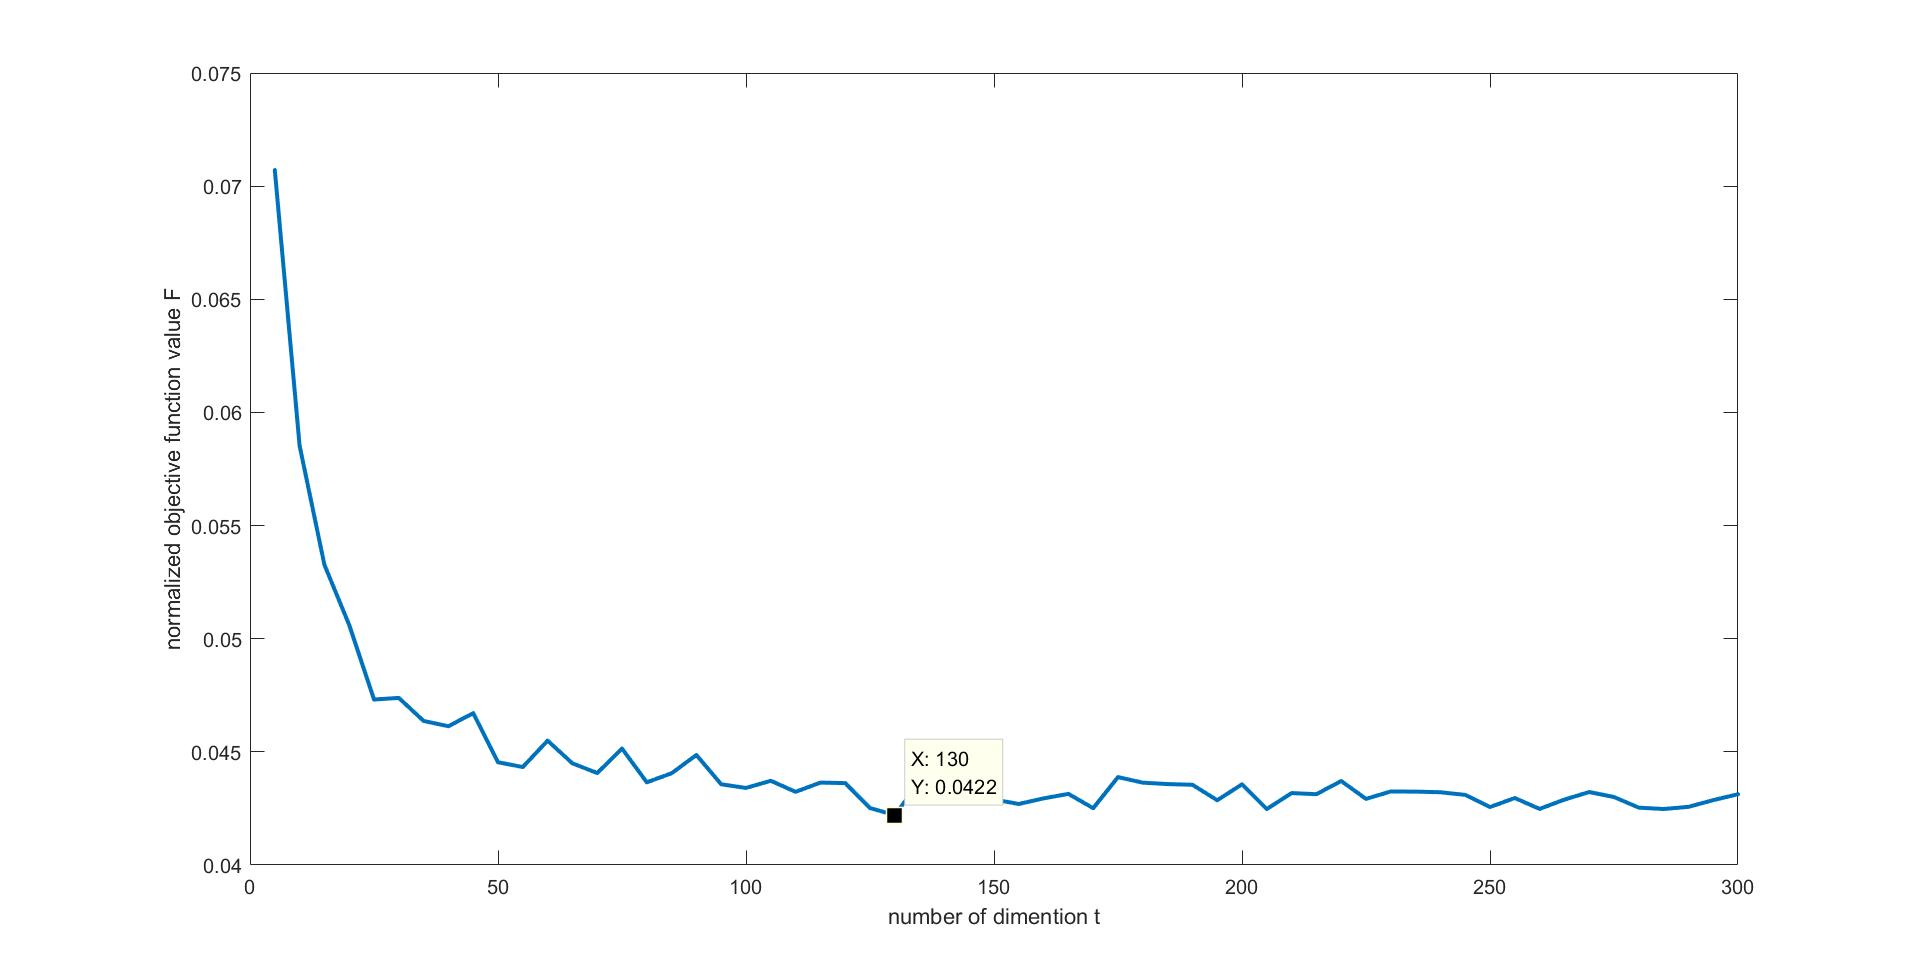
\includegraphics[width=0.50\textwidth]{result/norm_F.jpg}
        \caption{归一化的目标函数}
        \label{1}
        \end{figure}

        \begin{figure}[h]
        \centering
        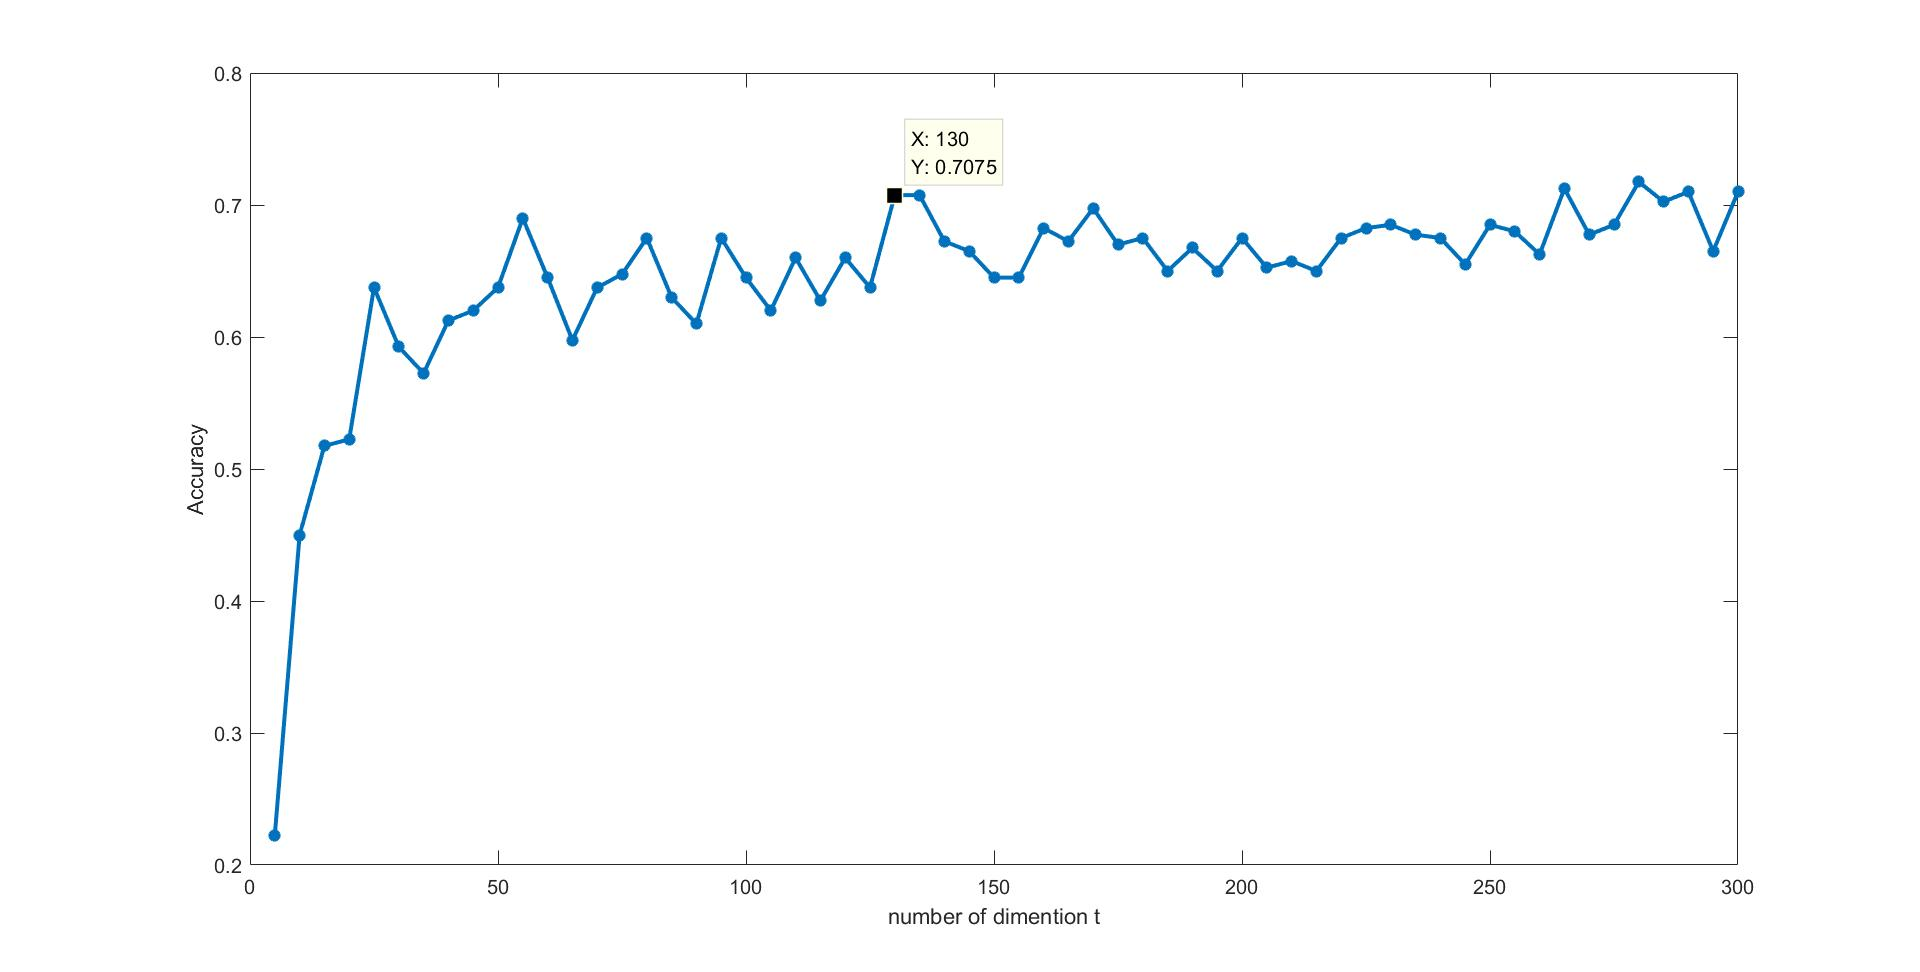
\includegraphics[width=0.50\textwidth]{result/acc.jpg}
        \caption{分类的准确率}
        \label{2}
        \end{figure}

        \begin{figure}[h]
        \centering
        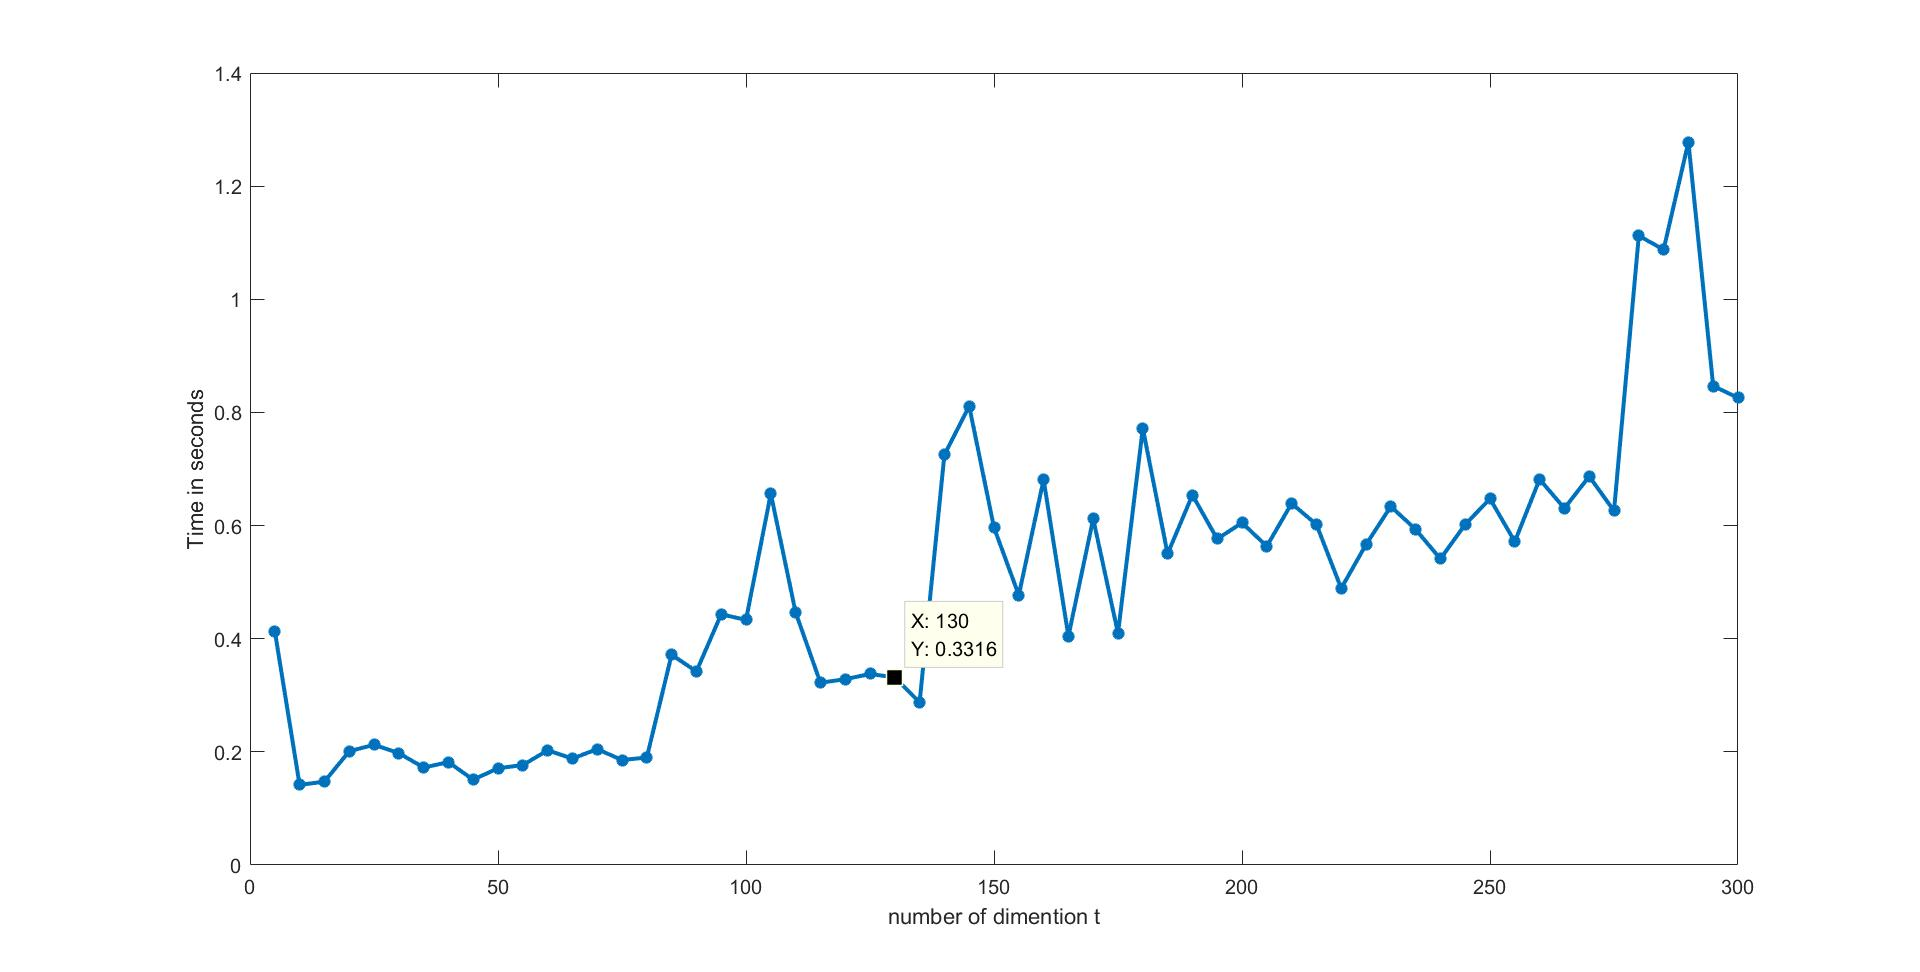
\includegraphics[width=0.50\textwidth]{result/time_RP.jpg}
        \caption{算法运行的总时间}
        \label{3}
        \end{figure}

    可以看出随着t的增长除了执行时间一直在增长之外,目标函数和准确率的变化趋势逐渐减小,从这次实验的结果看大概在维度是130的时候,目标函数和准确率可以达到几乎最优的程度,再继续增加t结果变化程度比较小,同时在这个维度执行时间也比较短。

    \subsection{思考与改进}
    因为这种基于随机投影的降维方法可解释性不是特别强,我们暂时没有想到怎样从精度上做改进,下面的改进思路主要都是在速度上的\\
    主要的三个改进思路分别是
    \begin{enumerate}
    \item 构造新的随机投影矩阵
    \item 使用mailman算法加速矩阵向量乘法
    \item 多次实验取最好的结果
    \end{enumerate}

    \subsubsection{构造新的随机投影矩阵}
    下面除了论文中随机投影矩阵的构造方法之外,另外使用三种随机投影矩阵的构造方法
    \begin{itemize}
    \item $\forall i,j \quad R_{i,j} \sim N(0,1)$
    \item 在本实验随机矩阵的基础上,使用稀疏矩阵,满足
    \begin{equation*}
    R_{ij} = \begin{cases} +\sqrt{3}/\sqrt{t},& \mbox{w.p. 1/6,} \\0, & \mbox{w.p. 2/3,} \\ -\sqrt{3}/\sqrt{t}, & \mbox{w.p. 1/6.}\end{cases}
    \end{equation*}
    \item Fast JL变换\\
    构造$\Phi = PHD$,其中$P \in R^{k \times d}, H,D \in R^{d \times d}$\\
    P的构造如下:
    \begin{equation*}
    P_{ij} = \begin{cases} N(0,1/q),& \mbox{w.p. q,} \\0, & \mbox{w.p. 1-q}\end{cases}\\
    q = min\Bigl\{ \theta \Bigl(\frac{log^2 n}{d}\Bigr),1 \Bigr\}
    \end{equation*}
    在本实验中q的取值大约为0.07左右,可以看出P非常稀疏,H是归一化的Hadamard矩阵,D是对角矩阵,对角线元素以1/2概率取-1或1.\\
    理论上FJLT的方法可以达到$\theta(nd/\varepsilon^2)$的时间复杂度,这里要求d是二的幂次,所以使用了64*64的ORL数据集
    \end{itemize}

    首先比较一下算法各个部分所用的时间,结果如\ref{time4}.
    \begin{figure}[h]
        \centering
        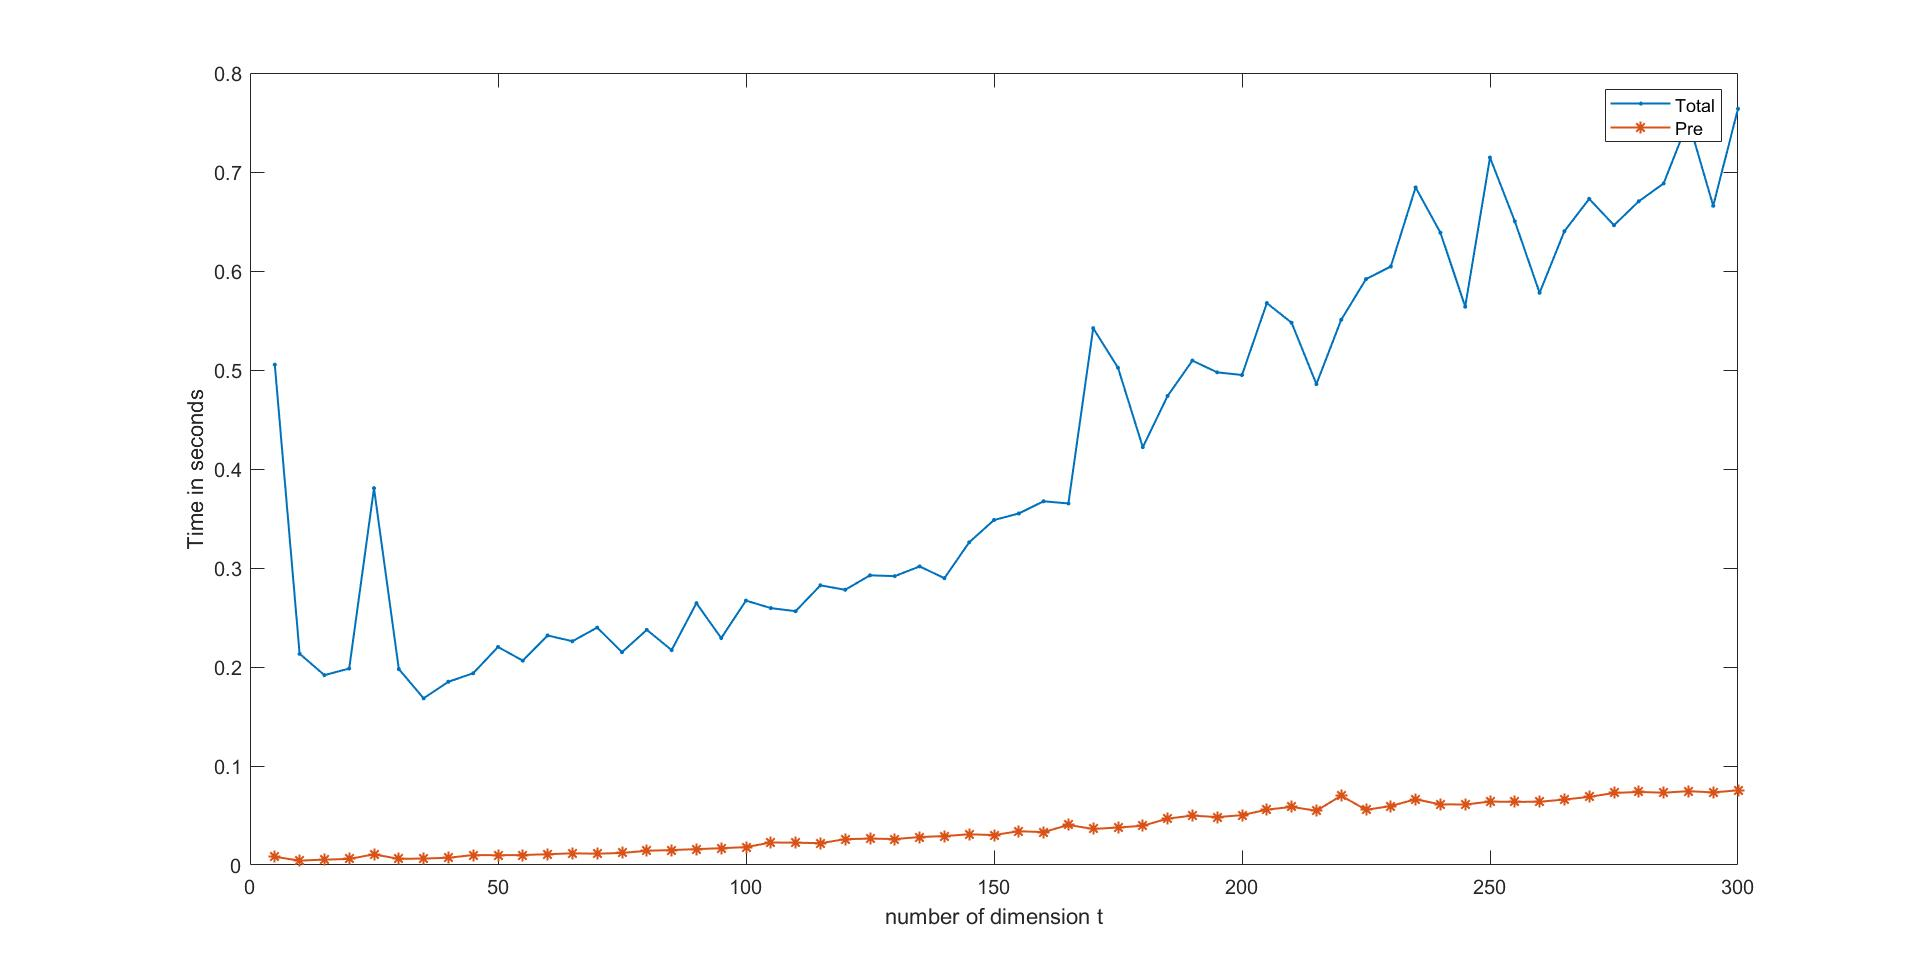
\includegraphics[width=0.50\textwidth]{result/total_pre.jpg}
        \caption{算法总时间和预处理时间}
        \label{time4}
    \end{figure}

    这里把除了k-means算法之外的计算时间称为预处理时间,可以看到k-means算法的时间是整个算法主要的时间开销,所以不再单独比较四种JL变换的预处理时间\\

    比较四种随机投影矩阵的分类准确率,结果如\ref{accu4}.
    \begin{figure}[h]
        \centering
        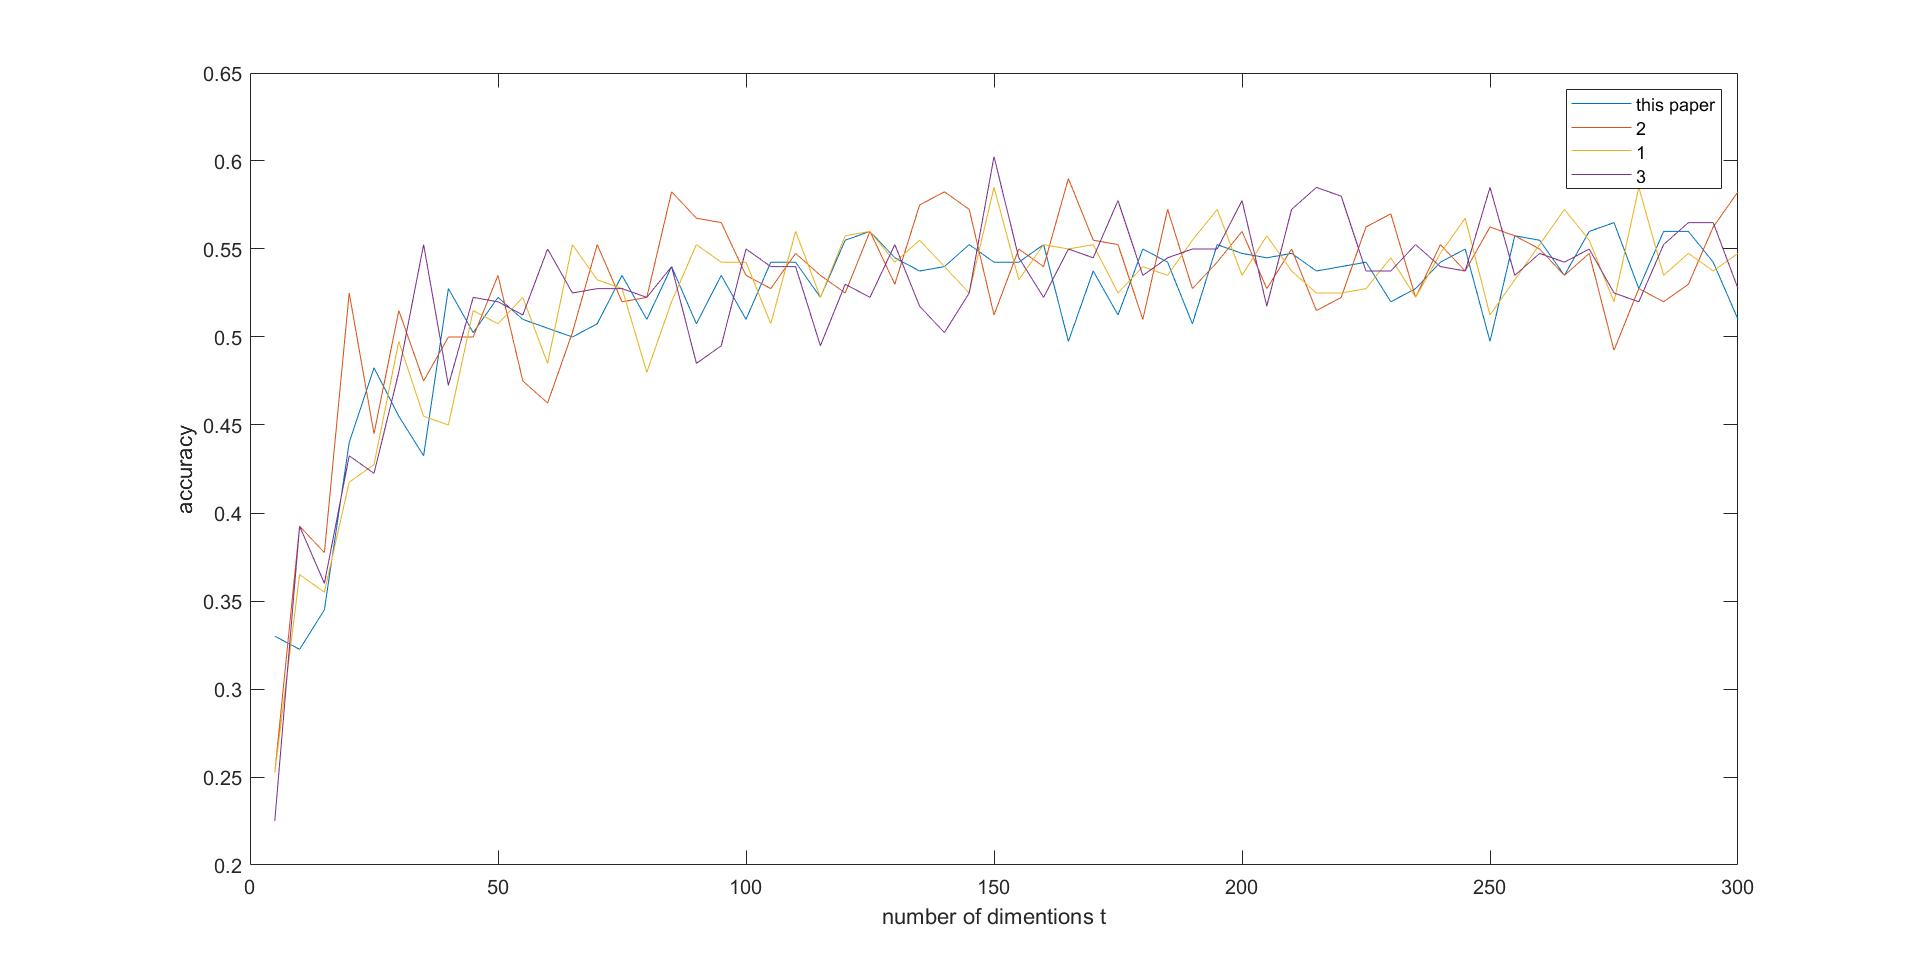
\includegraphics[width=0.50\textwidth]{result/accu.jpg}
        \caption{四种随机投影矩阵的分类准确率比较}
        \label{accu4}
    \end{figure}

    考虑随机性等原因,我们认为使用这四种随机投影矩阵进行降维并用在k-means中对于分类准确率影响不大.\\

    \subsubsection{使用mailman算法加速矩阵向量乘法}
    当矩阵A的每个元素只取固定的值时,mailman算法能够把矩阵向量乘法$A\vec{x}$的时间复杂度从$O(mn)$降到$O(mn/log(max{m,n}))$
    Mailman算法的核心思想是矩阵向量乘法$A\vec{x}$,其中$A \in R^{m \times n}, \vec{x}\in R^{n \times 1}$可以分解成以下形式\\
    \begin{equation*}
    A\vec{x} = \sum_{i=1}^n A^{(i)}x^{(i)}
    \end{equation*}
    其中,$A^{(i)}$表示A的第i列,$x^{(i)}$表示x的第i个元素,如果想象成是邮递员在送信,$A^{(i)}$就是地址,$x^{(i)}$是信,整个矩阵向量乘法就是邮递员遍历不同的地址送不同的信,但是因为地址是确定的,原始的乘法只是机械地走完全程,并没有考虑地址相同的情况。\\

    下面简单描述一下如何使用mailman算法计算矩阵向量乘法,这里不妨假设$ m = log_2^n$,并且$A(i,j) \in {0,1}$,如果不是可以把矩阵分成子矩阵或再进行扩展.
    构造两个新矩阵$U_{n}$和$n \times n$的矩阵P,$U_{n}$的每一列存储可能出现的由m个{0,1}组成的向量,那么A的每一列在$U_{n}$中都会出现。$P(i,j) = \delta(U^{(i)},A^{(j)})\quad \delta = 1 \quad \text{if} \quad U^{(i)} = A^{(j)}$,所以P只有n个非零元。
    \begin{align*}
    \because (U_{n}P)(i,j) &=\sum_{k=1}^n U_{n}(i,k)P(k,j)\\
    &=\sum_{k=1}^n U_{n}^{(k)}(i)\delta (U_{n}^{(k)},A^{(j)})\\
    &=A(i,j)\\
    \therefore A\vec{x} &=(UP)\vec{x} = U(P\vec{x})\\
    \end{align*}
    因为P只有n个非零元,计算$P\vec{x}$的时间复杂度为$O(n)$,利用二的幂次的性质,递归计算$U(P\vec{x})$的时间复杂度也为$O(n)$,更一般的情况下,在使用随机投影降维的算法中,理论上时间复杂度可以降低$max\{n,d\}$,但是不论是在mailman算法的原始文献中还是在随机投影降维的文章中,作者都表示实际无法达到理论效果,所以并没有对该算法进一步尝试。


    \section{基于SVD的特征选择}
    \label{sec:svdsec}
    尽管特征提取方法可以得到非常好的降维效果,但由于该方法得到的特征都是人为构造的,因而可解释性略差。
    相比之下,特征选择算法直接从原矩阵中抽取一些特征,我们可以清晰地看到哪些特征出现在了降维后的矩阵里(\autoref{sec:svdexp}),
    可解释性非常好。

    事实上,SVD和$k$-means聚类有着十分紧密的联系。我们知道,$X_{opt}$的秩至多为k,而$A_k$是$A$的最佳秩为k的估计,
    因此一个有趣的结论如下:
    \begin{align*}
        \Vert A_{\rho - k} \Vert_F^2 = \Vert A - A_k \Vert_F^2 \leq \Vert A - X_{opt} X_{opt}^T A \Vert_F^2
    \end{align*}
    
    在\cite{drineas1999clustering}中,作者证明了将$A$投影到其最佳$k$维子空间得到的$n \times k$矩阵$\tilde{A}=U_k \Sigma_k$后进行$k$-means聚类,可以
    得到一个最优聚类的2-approximation:
    \begin{align*}
        \Vert A - \tilde{X}_{opt} \tilde{X}_{opt}^T A \Vert_F^2 \leq 2 \min \Vert A - X X^T A \Vert_F^2
    \end{align*}

    这实际上是本小节中介绍的算法的出发点。在本算法中,我们将以上k个构造的特征
    替换为$\Theta(k \log(k / \epsilon) / \epsilon^2)$个实际的特征,得到一个$(2+\epsilon)$-approximate的结果。
    
    \subsection{算法概述}
    \begin{algorithm}[htb]
    \caption{用于$k$-means聚类的特征选择算法}
    \label{SVD}
        \begin{algorithmic}[1] %这个1 表示每一行都显示数字
        \REQUIRE ~~\\ %算法的输入参数:Input
            矩阵 $ A \in R^{n \times d}$, 类的数目k, 误差因子 $\varepsilon \in (0, 1)$, $\gamma$近似的k-means算法。 \\
        \ENSURE ~~\\ %算法的输出:Output
            矩阵 $ X_{\tilde{\gamma}} $ 表示聚类结果。

        \STATE 设置目标维度 $ r = \Theta(k \log(k / \epsilon) / \epsilon^2)$。

        \STATE 计算前$k$个右奇异向量$V_k$。

        \STATE 计算\textbf{杠杆得分}$p_i$,对于$i=1, \dots, d$,$p_i = \Vert (V_k)_{(i)} \Vert_2^2 / k$。
        \label{compls}

        \STATE 进行$r$次\textit{有放回}的采样,每一次以$p_i$的概率保留第i个特征,并将其乘以系数$(rp_i)^{-1/2}$。

        \STATE 在上一步产生的$n \times r$矩阵$\tilde{A}$上运行$\gamma$近似的$k$-means算法,返回矩阵$X_{\tilde{\gamma}}$。

        \end{algorithmic}
    \end{algorithm}

    可以看到,该算法是通过随机采样的方式进行特征选择的。特别地,以上方法称为\textbf{杠杆得分采样}(\textit{leverage score sampling})。
    杠杆得分是在该算法第3步计算出的,它代表了特征的“重要性”,在\cite{Mahoney2009cur}中有对其清晰的解释:

    根据SVD分解,我们可以将A的第j列表示为左奇异向量的线性组合:$A^j=\sum_{i=1}^{r} (\sigma_i u^i)v_j^i$,其中$v_j^i$表示第j个右奇异向量的第i个元素。
    我们也可以用前k个左奇异向量估计$A^j=\sum_{i=1}^{k} (\sigma_i u^i)v_j^i$。因此,特征的重要性可以根据其在前k个左奇异向量组成的线性空间中的长度决定,即:
    $\pi_j = \frac{1}{k} \sum_{i=1}^{k} (v_j^i)^2$,此处除以k是为了归一化。

    可以证明,以上算法运行于近似比为$\gamma$,失败率为$\delta_\gamma$的$k$-means聚类算法上时,可以以
    至少$0.5-\delta_\gamma$的概率得到$(1+(1+\epsilon)\gamma)$近似的聚类结果。降维算法中最复杂的运算为
    求前k个右奇异向量,因此时间复杂度为$O(\min(nd^2, n^2d))$。

    \subsection{理论推导}
    本小节对以上特征选择算法的PAC-界给出理论推导\cite{boutsidis2009unsupervised,boutsidis2014randomized}。

    \newtheorem{thm}{\bf 定理}[]
    \begin{thm}
    \label{thmsvd}
        按照\autoref{SVD}的得到的聚类结果$X_{\tilde{\gamma}}$,以至少
        $0.5-\delta_\gamma$的概率满足:
        $$
            \Vert A - X_{\tilde{\gamma}} X_{\tilde{\gamma}^T} A \Vert_F^2 \leq (1 + ( 1+\epsilon ) \gamma ) \Vert A - X_{opt} X_{opt}^T A \Vert_F^2
        $$
    \end{thm}

    为了证明以上定理,先给出以下两个概念:

    \textbf{采样矩阵}$S$是一个$d \times r$矩阵,它是这样构造出的:在\autoref{SVD}的有放回采样过程中,
    每次若第$i$个特征被选中,则将$e_i$(第i项为1,其它均为0的列向量)加入到矩阵$S$中都会出现。

    \textbf{缩放矩阵}$D$是一个$r \times r$对角矩阵,在\autoref{SVD}采样的过程中,若第$t$次采样,第$i$个特征被
    选中,则将第$t$列的对角项设为$1 / \sqrt{rp_i}$。

    有了以上两个定义,下面给出一个引理\cite{boutsidis2009unsupervised}:
    \newtheorem{lemma}{\bf 引理}[]
    \begin{lemma}
    \label{lmsvd}
        若$r$满足\autoref{SVD}中的条件,则以下四个语句以至少0.5的概率同时成立:
        \begin{enumerate}
            \item $\Vert V_k^T S D \Vert_2 = \sigma_{max}(V_k^T S D) \leq \sqrt{1 + \lambda}$。
            \item $\Vert (V_k^T S D)^+ \Vert_2 = 1 / \sigma_{min}(V_k^T S D) \leq \sqrt{1 / (1 - \lambda)}$。
            \item $V_k^T S D$满秩。
            \item $A_k = (ASD) (V_k^T SD)^+ V_k^T + E$,其中$\Vert E \Vert_F \leq \mu \Vert A - A_k \Vert_F$。
        \end{enumerate}
        其中,$\lambda$和$\mu$为给定的常数\cite{boutsidis2009unsupervised}。
        
    \end{lemma}

    \begin{proof}
        首先证明前两条:

        定义随机向量$y \in R^k$如下:对于$i = 1, \dots, d$,P[$y=y_i$] $= p_i$,其中$y_{i}=(1 / \sqrt{p_{i}})\left(V_{k}^{T}\right)^{(i)}$。那么,
        $S$和$D$的定义表明:$V_{k}^{T} S D D S^{T} V_{k}=\frac{1}{r} \sum_{i=1}^{d} y_{i} y_{i}^{T}$,
        \(p_{i}=\left\|\left(V_{k}^{T}\right)^{(i)}\right\|_{2} / k\)使得\(\|y\|_{2} \leq \sqrt{k}\).
        又有\(\left.E\left[y y^{T}\right]=\sum_{i=1}^{d} p_{i} \frac{1}{\sqrt{p_{i}}}\left(V_{k}^{T}\right)^{(i)} \frac{1}{\sqrt{p_{i}}}\left(V_{k}^{T}\right)^{(i)}\right)^{T}=V_{k}^{T} V_{k}=I_{k}\)。
        运用\cite{rudelson2007sampling}中的定理3.1,结合Markov不等式,得到对于足够大的$c_0$,以至少$1-1/6$的概率:
        $$
        \left\|V_{k}^{T} S D D S^{T} V_{k}-I_{k}\right\|_{2} \leq 6 c_{0} \sqrt{k \log (r) / r}
        $$
        
        根据矩阵摄动理论\cite{boutsidis2009unsupervised},有:
        $$
        \left\|V_{k}^{T} S D D S^{T} V_{k}-I_{k}\right\|_{2}=\left|\sigma_{i}^{2}\left(V_{k}^{T} S D\right)-1\right| \leq 6 c_{o} \sqrt{k \log (r) / r}
        $$

        前两条因此得证。为了证明第三条,我们只需证明$V_k^T S D$的第$k$个奇异值为正。事实上,
        $\epsilon$的取值和引理的第二条已经保证了这一结果。

        为了证明第四条,我们首先有:
        $$
        \begin{aligned}\left\|A_{k}-A S D\left(V_{k}^{T} S D\right)^{+} V_{k}^{T}\right\|_{F} &=\left\|A_{k}-A_{k} S D\left(V_{k}^{T} S D\right)^{+} V_{k}^{T}-A_{\rho-k} S D\left(V_{k}^{T} S D\right)^{+} V_{k}^{T}\right\|_{F} \\ & \leq\left\|A_{k}-A_{k} S D\left(V_{k}^{T} S D\right)^{+} V_{k}^{T}\right\|_{F}+\left\|A_{\rho-k} S D\left(V_{k}^{T} S D\right)^{+} V_{k}^{T}\right\|_F \end{aligned}
        $$

        以上第一步,我们将$A$替换为$A_k + A_{\rho - k}$,第二步运用了矩阵范数的三角不等式。我们将第一项设为$\theta_1$,第二项为$\theta_2$,则有:
        $$
        \begin{aligned} \theta_{1} &=\left\|A_{k}-U_{k} \Sigma_{k} V_{k}^{T} S D\left(V_{k}^{T} S D\right)^{+} V_{k}^{T}\right\|_{F} \\ &=\left\|A_{k}-U_{k} \Sigma_{k} I_{k} V_{k}^{T}\right\|_{F}=0 \end{aligned}
        $$
        $$
        \begin{aligned} \theta_{2} &=\left\|U_{\rho-k} \Sigma_{\rho-k} V_{\rho-k}^{T} S D\left(V_{k}^{T} S D\right)^{+} V_{k}^{T}\right\|_{F} \\ & \leq\left\|\Sigma_{\rho-k} V_{\rho-k}^{T} S D\left(V_{k}^{T} S D\right)^{+}\right\|_{F} \end{aligned}
        $$

        对于后一项,如果前三项以至少$1-1/6$的概率成立,则以至少$1-1/3$的概率有:
        $$
        \left\|\Sigma_{\rho-k} V_{\rho-k}^{T} S D\left(V_{k}^{T} S D\right)^{+}\right\|_{F} \leq(\epsilon \sqrt{6 /\left(2 c_{1} c_{o}^{2} \log \left(c_{1} c_{o}^{2} k / \epsilon^{2}\right)\right)}+\sqrt{6 \lambda^{2} /(1-\lambda)})\left\|A-A_{k}\right\|_{F}
        $$

        因此,根据union bound,所有四条引理以至少$1-1/6-1/3= 1-1/2$的概率成立。

        证毕。
    \end{proof}

    有了以上引理,我们可以对定理\autoref{thmsvd}给出证明:
    \begin{proof}
        首先,我们将$A$分为$A=A_k + A_{\rho-k}$,再运用矩阵范数勾股定理\cite{boutsidis2014randomized},则有:
        $$
        \left\|A-X_{\tilde{\gamma}} X_{\tilde{\gamma}}^{T} A\right\|_{F}^{2}=\left\|\left(I-X_{\tilde{\gamma}} X_{\tilde{\gamma}}^{T}\right) A_{k}\right\|_{F}^{2}+\left\|\left(I-X_{\tilde{\gamma}} X_{\tilde{\gamma}}^{T}\right) A_{\rho-k}\right\|_{F}^{2}
        $$

        与引理的证明相同,我们将第一项称为$\theta_3^2$,第二项称为$\theta_4^2$。对于第二项,由于$I-X_{\tilde{\gamma}} X_{\tilde{\gamma}}^T$是投影矩阵,
        去掉它不会使范数增大,再结合本章开头的结论,有:
        $$
        \theta_4^2 \leq F_{opt}
        $$

        下面讨论第一项的界:
        $$
        \begin{aligned} \theta_{3} & \leq\left\|\left(I-X_{\tilde{\gamma}} X_{\tilde{\gamma}}^{T}\right) A S D\left(V_{k} S D\right)^{+} V_{k}^{T}\right\|_{F}+\|E\|_{F} \\ & \leq\left\|\left(I-X_{\tilde{\gamma}} X_{\tilde{\gamma}}^{T}\right) A S D\right\|_{F}\left\|\left(V_{k} S D\right)^{+}\right\|_{2}+\|E\|_{F} \\ & \leq \sqrt{\gamma}\left\|\left(I-X_{o p t} X_{o p t}^{T}\right) A S D\right\|_{F}\left\|\left(V_{k} S D\right)^{+}\right\|_{2}+\|E\|_{F} \\ & \leq \sqrt{\gamma}\left\|\left(I-X_{o p t} X_{o p t}^{T}\right) A S D\left(V_{k} S D\right)^{+}\right\|_{F}\left\|\left(V_{k} S D\right)\right\|_{2}\left\|\left(V_{k} S D\right)^{+}\right\|_{2}+\|E\|_{F} \\ &=\sqrt{\gamma}\left\|\left(I-X_{o p t} X_{o p t}^{T}\right) A S D\left(V_{k} S D\right)^{+} V_{k}^{T}\right\|_{F}\left\|\left(V_{k} S D\right)\right\|_{2}\left\|\left(V_{k} S D\right)^{+}\right\|_{2}+\|E\|_{F} \end{aligned}
        $$

        其中,第一步我们使用了引理\autoref{lmsvd}、三角不等式和投影矩阵的性质,第二步我们使用了
        数学符号约定(\autoref{sec:symbols})里的结果,第三步是基于以下结论:
        $$
        \left\|\left(I-X_{\tilde{\gamma}} X_{\tilde{\gamma}}^{T}\right) A S D\right\|_{F}^{2} \leq \gamma \min _{X \in \mathcal{X}}\left\|\left(I-X X^{T}\right) A S D\right\|_{F}^{2} \leq \gamma\left\|\left(I-X_{o p t} X_{o p t}^{T}\right) A S D\right\|_{F}^{2}
        $$

        在第四步和第五步,我们分别加入了一些不影响矩阵范数的项。

        我们设$\theta_5 = \left\|\left(I-X_{o p t} X_{o p t}^{T}\right) A S D\left(V_{k} S D\right)^{+} V_{k}^{T}\right\|_{F}$,则可以有如下对其的讨论:

        $$
        \begin{aligned} \theta_{5} & \leq\left\|\left(I-X_{o p t} X_{o p t}^{T}\right) A_{k}\right\|_{F}+\left\|\left(I-X_{o p t} X_{o p t}^{T}\right) E\right\|_{F} \\ & \leq\left\|\left(I-X_{o p t} X_{o p t}^{T}\right) A V_{k} V_{k}^{T}\right\|_{F}+\|E\|_{F} \\ & \leq(1+\mu) \sqrt{F_{o p t}} \end{aligned}
        $$

        在第一步,我们运用了引理\autoref{lmsvd}和三角不等式,第二步我们将前一项的$A_k$展开,
        后一项去掉了投影矩阵,第三步我们去掉了投影矩阵并使用了本章开头的结论。将上述结论带回$\theta_3$,则:
        $$
        \theta_{3} \leq \sqrt{\gamma}(\sqrt{\frac{1+\lambda}{1-\lambda}}(1+\mu)+\mu) \sqrt{F_{o p t}}
        $$

        易知,括号内的部分小于$\sqrt{1 + \lambda}$,由此,我们得到:
        $$
        \theta_{3}^{2} \leq \gamma(1+\epsilon) F_{o p t}
        $$

        由于定理\autoref{thmsvd}失效当且仅当引理\autoref{lmsvd}或近似$k$-means算法失效,
        两者概率至多为$0.5+\delta_\gamma$。综上,定理得证。
    \end{proof}
    \subsection{实验验证}
    \label{sec:svdexp}
    我们首先在原文所使用的NIPS数据集\cite{chechik2007eec}上进行了验证。
    数据集为一个$183 \times 6314$的文本-词项矩阵,包含了2001-2003年发表在NIPS上的文章,分为神经科学、学习理论、控制和强化学习三类。
    \autoref{fig:svdfeat}和\autoref{fig:nipsp}表示了我们的实验结果。

    \begin{figure}[H]
        \centering
        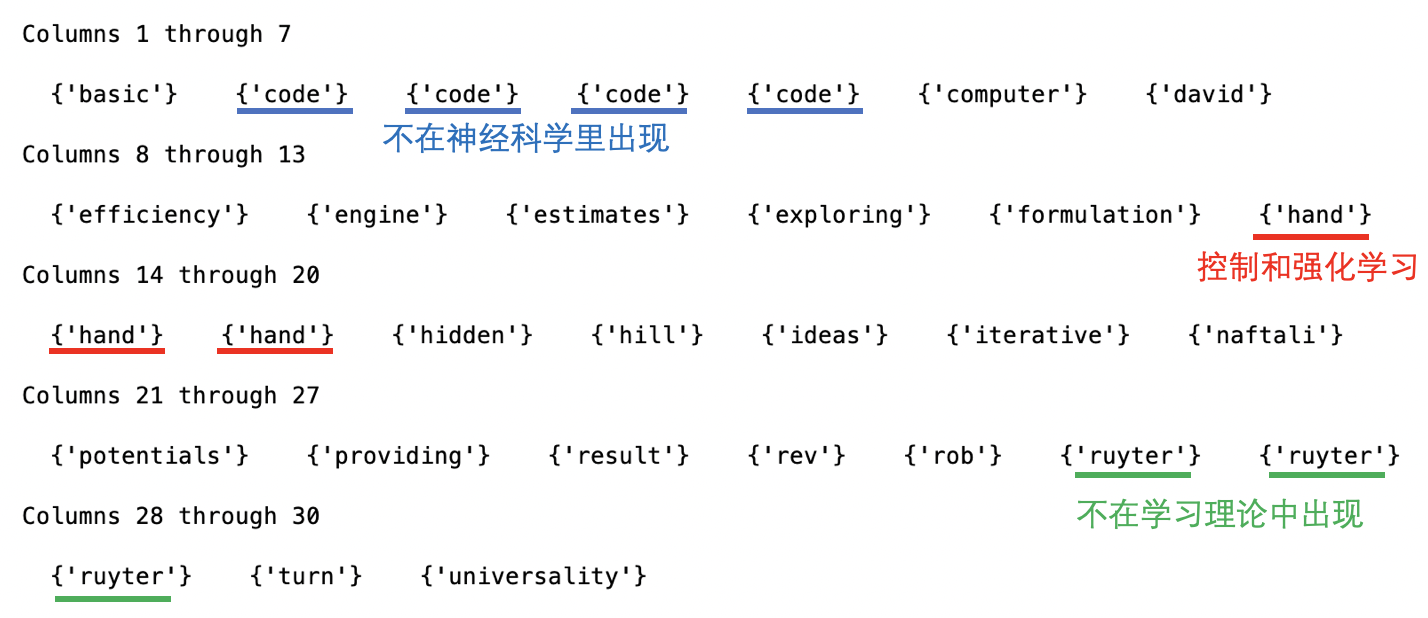
\includegraphics[width=0.8\textwidth]{result/words.png}
        \caption{\autoref{SVD}选出的特征}
        \label{fig:svdfeat}
    \end{figure}

    从\autoref{fig:svdfeat}可以看出,有一些特征被重复选了多次,根据领域知识可以知道,
    这些特征恰恰是不同领域中具有代表性的词语,这说明我们的选择算法是有效的。此外,我们可以直观地
    看到算法选出的特征,也说明了特征选择算法良好的可解释性[\autoref{sec:svdsec}]。

    \begin{figure}[H]
        \centering
        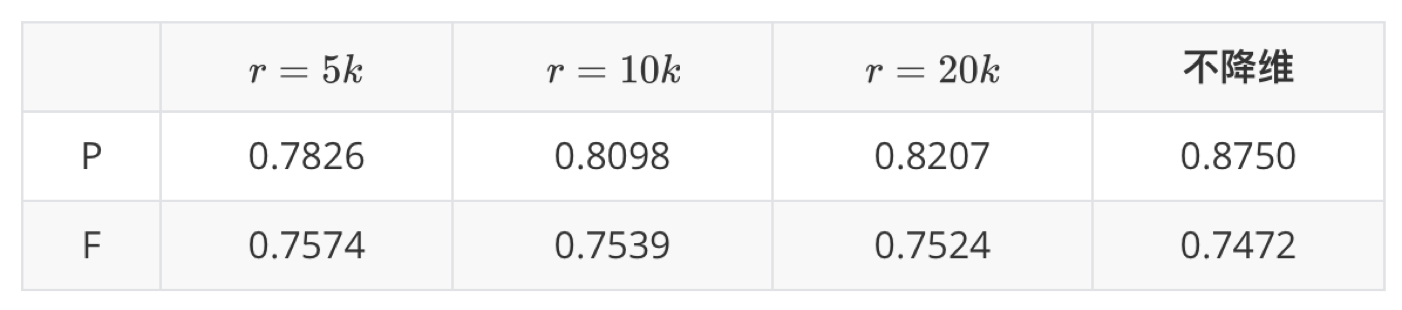
\includegraphics[width=0.8\textwidth]{result/nipsp.png}
        \caption{\autoref{SVD}的分类正确率和目标函数值}
        \label{fig:nipsp}
    \end{figure}

    从\autoref{fig:nipsp}可以看出,降维后聚类的正确率与不降维的差距不大。事实上,尽管
    我们的算法要求目标维度$ r = \Theta(k \log(k / \epsilon) / \epsilon^2)$,但是
    在实验中选择远小于该值的$r$就可以良好地完成降维任务。

    \subsubsection{两种方法的比较}
        我们还在ORL数据集上对特征选择和特征提取算法的正确率和执行时间进行了比较:
        \begin{figure}[H]
            \centering
            \begin{subfigure}{.5\textwidth}
                \centering
                \includegraphics[width=1.0\linewidth]{result/precision.jpg}
                \caption{正确率}
            \end{subfigure}%
            \begin{subfigure}{.5\textwidth}
                \centering
                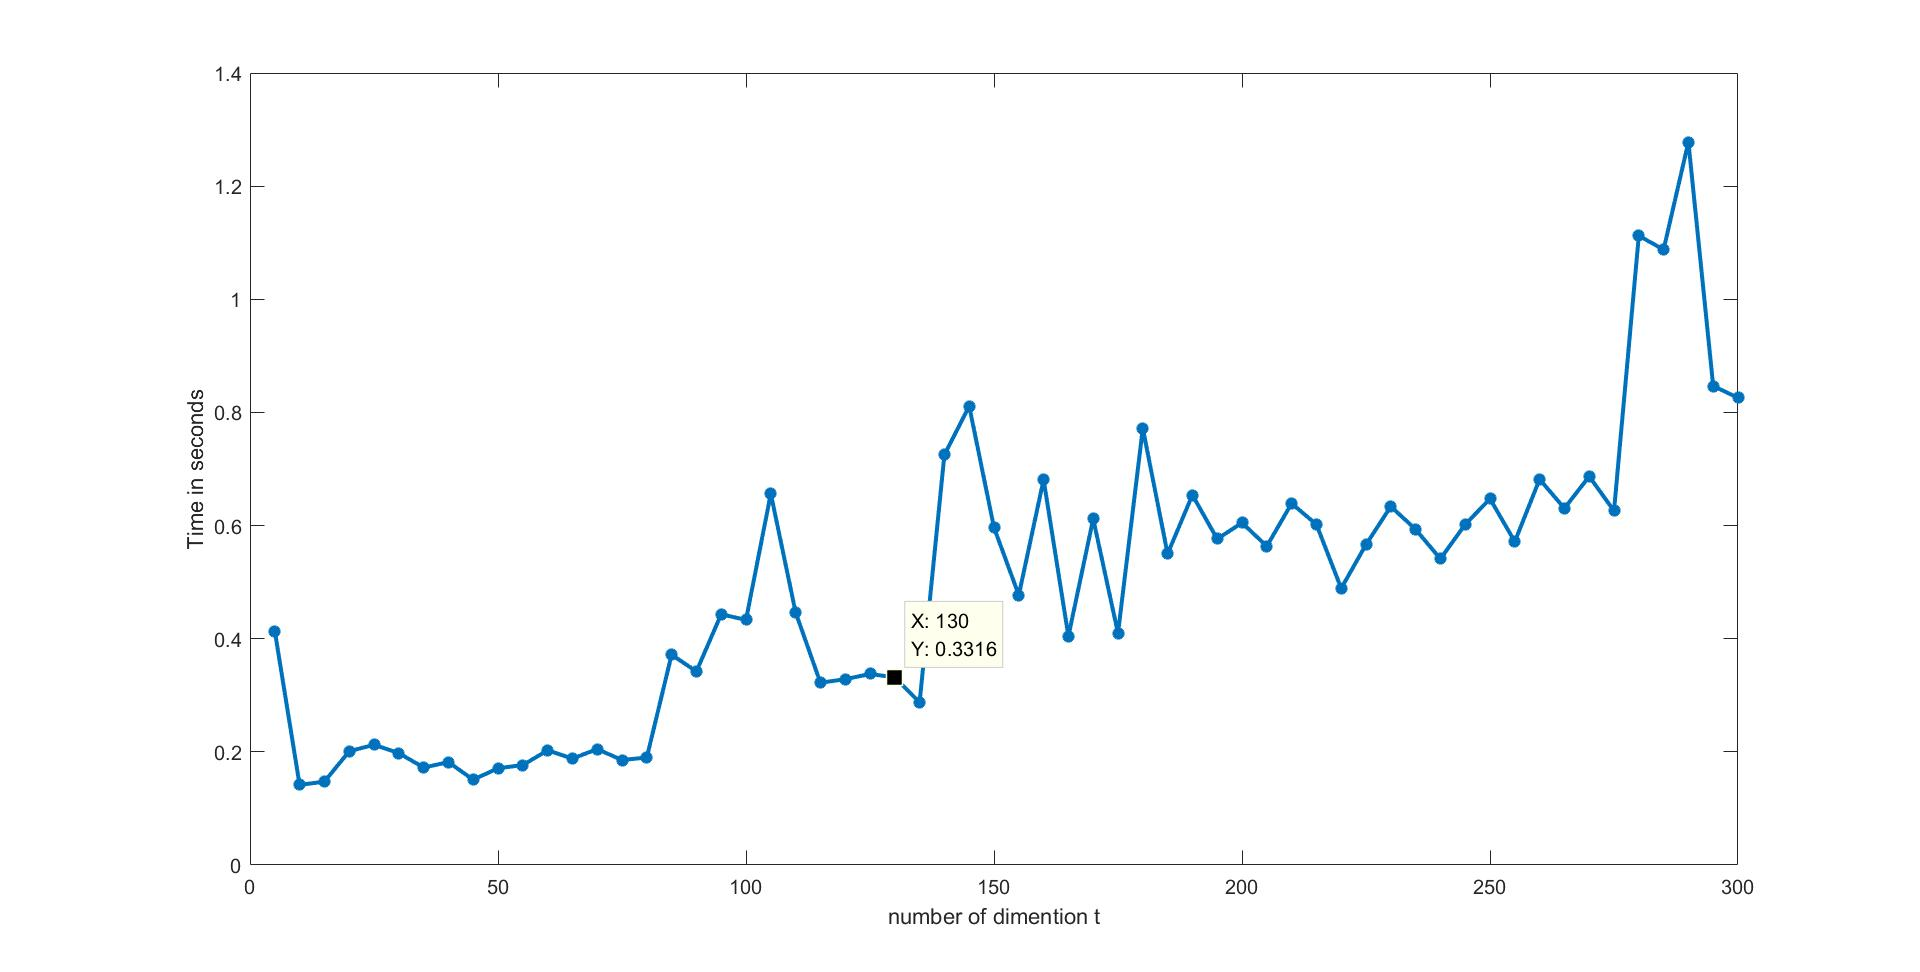
\includegraphics[width=1.0\linewidth]{result/time.jpg}
                \caption{执行时间}
            \end{subfigure}
            \caption{两种降维算法的比较}
            \label{fig:cmp}
        \end{figure}

        比较的结果非常直观,相对来讲,基于SVD的特征选择算法比基于随机投影的特征提取算法正确率
        稍高,但执行时间则长了很多。这是由于SVD运算的时间复杂度是三次方量级。事实上,在实际的
        大数据计算中,我们难以承受对巨大的矩阵进行SVD分解的时间和空间开销\cite{blum2020foundations,halko2011finding,halko2011finding}。
    
    \subsection{思考与改进}
    在本小节中,针对上一小节实验中发现的SVD执行速度慢的问题,我们利用一种近似SVD算法进行改进[\autoref{sec:appsvd}],
    我们还将就杠杆得分函数的有效性进行讨论[\autoref{sec:lsdis}],最后,我们将我们的降维方法与确定性的
    PCA方法进行比较[\autoref{sec:cmppca}]。

    \subsubsection{用近似算法加速SVD计算}
    \label{sec:appsvd}
    在\autoref{sec:svdexp}中,我们发现SVD计算非常费时,影响了特征选择算法的执行速度。
    事实上,学术界对加速SVD计算的方法已经有了深入的研究\cite{halko2011finding},在本小节中,我们介绍一种
    随机算法来加速SVD计算\cite{szlam2014implementation},下面概述其计算步骤:
    \begin{algorithm}[H]
    \caption{近似SVD算法}
    \label{redsvd}
        \begin{algorithmic}[1] %这个1 表示每一行都显示数字
        \REQUIRE ~~\\ %算法的输入参数:Input
            矩阵 $ A \in R^{n \times d}$, 参数k。
        \ENSURE ~~\\ %算法的输出:Output
            近似的前k个奇异值和奇异向量。
        \STATE 将$A$作用于$k$个独立同分布的随机向量得到$B$,可以证明,$B$以很大概率覆盖A的列向量空间\cite{halko2011finding}。
        \STATE 利用Gram-Schmidt等方法得到$B$的标准正交基$Q$。
        \STATE 由于$Q$几乎覆盖了$A$的列向量空间,所以有$A \approx Q Q^T A = Q (Q^T A)$。
        \STATE 计算$Q^T A$的SVD:U、S、V,因为它只有$k \times n$维,所以计算很快。
        \STATE $A \approx Q Q^T A = (QU) S V^T$。
        \end{algorithmic}
    \end{algorithm}

    我们利用\autoref{redsvd}替换\autoref{SVD}中计算前k个右奇异向量的过程,可以看到,它的执行时间
    与随机投影算法已经基本相同,主要受限于$k$-means的执行速度,而它的准确率却几乎没有下降。
    \begin{figure}[H]
        \centering
        \begin{subfigure}{.5\textwidth}
            \centering
            \includegraphics[width=1.0\linewidth]{result/accuracy_rand.jpg}
            \caption{正确率}
        \end{subfigure}%
        \begin{subfigure}{.5\textwidth}
            \centering
            \includegraphics[width=1.0\linewidth]{result/time_rand.jpg}
            \caption{执行时间}
        \end{subfigure}
        \caption{利用近似SVD加速后的效果}
        \label{fig:3cmp}
    \end{figure}


    \subsubsection{关于杠杆得分采样效果的讨论}
    \label{sec:lsdis}
    在\autoref{fig:nipsp}中,我们得出的结论是特征选择算法的正确率很高,但这是
    我们进行了一百次重复实验后取目标函数最大的聚类结果得到的。实际上,这一百次实验的正确率分布如\autoref{fig:rescale}

    \begin{figure}[H]
        \centering
        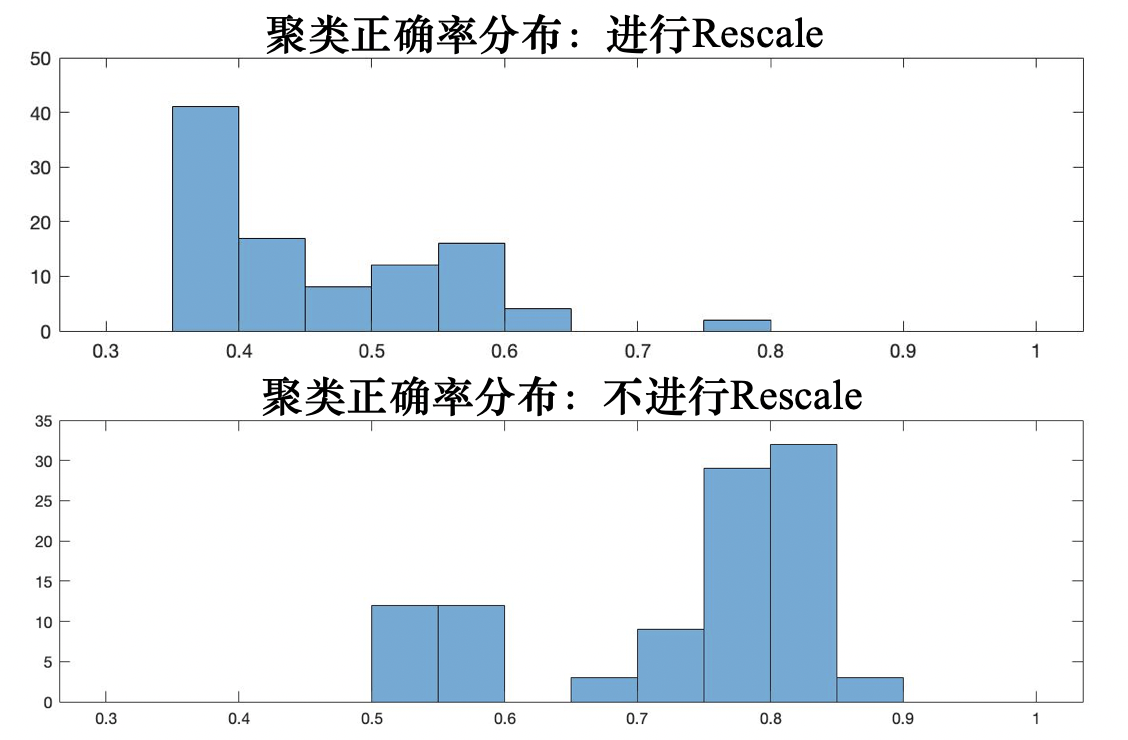
\includegraphics[width=0.6\textwidth]{result/nipscmp.png}
        \caption{进行与不进行rescale的正确率分布}
        \label{fig:rescale}
    \end{figure}




    \subsubsection{与确定性算法的比较}
    \label{sec:cmppca}

    \section{结论}

\addcontentsline{toc}{section}{参考文献}
\nocite{*} % So we don't need to explicitly cite them
\bibliographystyle{plain}
\bibliography{ref}
\end{document} 